\documentclass[12pt,a4paper,oneside,english]{book}
\usepackage[linesnumbered,ruled,vlined,english,onelanguage]{algorithm2e}
%\usepackage{cite}

\usepackage{minitoc}
\usepackage[utf8]{inputenc}
\usepackage[T1]{fontenc}
\usepackage[english]{babel}
\usepackage{amsmath}
\usepackage{amsfonts}
\usepackage{amssymb}
\usepackage{graphicx}
%\usepackage{subfig}
\usepackage{subcaption}
\usepackage{fancyhdr}
\usepackage{appendix}
\usepackage{hyphenat}
\usepackage{pdfpages}
\usepackage{lettrine}
\usepackage{hyperref}
\usepackage[table]{colortbl}
\usepackage{float}
\usepackage{csquotes}

\usepackage[sorting=none,defernumbers=true]{biblatex}
\addbibresource{references.bib}
\addbibresource{webography.bib}

\usepackage{array,multirow,makecell}
\newcolumntype{C}[1]{>{\arraybackslash}p{#1}}

\usepackage{enumitem}
\setlist{leftmargin=*,itemsep=0pt}

\usepackage{centernot}

\usepackage{quotchap}
\makeatletter
\renewcommand{\@makechapterhead}[1]{
 \chapterheadstartvskip
 {\size@chapter{\sectfont\raggedright
 {\chapnumfont
 \ifnum \c@secnumdepth >\m@ne
 \if@mainmatter\thechapter
 \fi\fi
 \par\nobreak}
 {\raggedright\advance\leftmargin10em\interlinepenalty\@M #1\par}}
 \nobreak\chapterheadendvskip}}
\makeatother
\renewcommand*{\chapterheadendvskip}{\vspace{1cm}}
\renewcommand*{\chapterheadstartvskip}{
  \if@mainmatter
    \vspace{-100pt}% spacing for \chapter
  \else
    \vspace{50pt}% spacing for \chapter*
  \fi}


\usepackage{geometry}
\geometry{hmargin=2.5cm,vmargin=2.5cm}

\pagestyle{fancyplain}
\lhead{\fancyplain{}{\nouppercase{\textit{\leftmark}}}}
\chead{\fancyplain{}{}}
\rhead{\fancyplain{}{}}
\lfoot{\fancyplain{}{}}
\cfoot{\fancyplain{}{}}
\rfoot{\fancyplain{\thepage}{\thepage}}
\renewcommand{\headrulewidth}{1pt}
\renewcommand{\footrulewidth}{1pt}

\renewcommand{\thesection}{\arabic{section}}

\usepackage{titlesec}
\titleformat{\paragraph}{\fontsize{11}{10}\bfseries}{\theparagraph}{1em}{}
\titlespacing*{\paragraph}{0pt}{10pt plus 2pt minus 0pt}{0pt plus 2pt minus 0pt}

\setcounter{secnumdepth}{4}
\setcounter{tocdepth}{4}

\usepackage{array}
\usepackage{multirow}
\addto\captionsfrench{\def\tablename{\textsc{Tableau}}}

%\DefineBibliographyStrings{french}{urlseen = {},}

\setlength{\parskip}{8pt}
\usepackage{setspace}

\usepackage{url}

\usepackage{hyperref}
% Comment before printing to remove links' colors
\definecolor{darkblue}{rgb}{0.0, 0.0, 0.5}
\hypersetup{
 colorlinks,
 linktocpage=true,
 linkcolor={darkblue},
 citecolor={darkblue},
 urlcolor={blue}}

\sloppy

\author{You}
\title{PFE Report}

%--------------------------------------------------------------------------
%--------------------------------------------------------------------------
%--------------------------------------------------------------------------

\begin{document}

\pagenumbering{gobble}

\includepdf[pages=-]{FrontPage.pdf}
\dominitoc
\mtcsettitle{minitoc}{Plan}
\mtcsetrules{*}{off}

\chapter*{Dedication}

    \newlength{\originalparskip}
    \setlength{\originalparskip}{\parskip}

    \setlength{\parskip}{1cm}
    \setstretch{1.2}
    \begin{center}
    {\itshape
    This work is dedicated to the individuals .... 
    }
    \end{center}
    \setlength{\parskip}{\originalparskip}
    \setstretch{1}
\chapter*{Acknowledgements}
    \setlength{\parskip}{1cm}
    \setstretch{1.2}
    Acknowledging the debts of gratitude accumulated during this project ....
    \setlength{\parskip}{\originalparskip}
    \setstretch{1}


\chapter*{Abstract}
\setstretch{1.2}
\normalsize{
Your abstract here
}

\medskip
{\noindent \textbf{Keywords: your keywords here} }
\setstretch{1}
\chapter*{Résumé}
\setstretch{1.2}
\normalsize{
Votre résumé ici
}

\medskip
{\noindent \textbf{Mots-clés: vos mots-clés ici} }
\setstretch{1}

% This helps you know how many pages in each chapter to balance your report
% Don't forget to comment it in the end

\noindent
Chapter 1 has \the\numexpr\getpagerefnumber{chap:2nd}-\getpagerefnumber{chap:1st}\relax\space pages \newline
Chapter 2 has \the\numexpr\getpagerefnumber{chap:3rd}-\getpagerefnumber{chap:2nd}\relax\space pages \newline
Chapter 3 has \the\numexpr\getpagerefnumber{chap:4th}-\getpagerefnumber{chap:3rd}\relax\space pages \newline
Chapter 4 has \the\numexpr\getpagerefnumber{conclusion}-\getpagerefnumber{chap:4th}\relax\space pages \newline


\frontmatter
\spacing{1}
\tableofcontents
\newpage

\listoffigures \mtcaddchapter 
\newpage 

\listoftables
\newpage

\spacing{1.4}

\chapter*{List of acronyms}

\begin{itemize}
\item \textbf{IT.} Information Technology

\end{itemize}

\mainmatter

\chapter*{General Introduction}
\addcontentsline{toc}{chapter}{General Introduction}
\markboth{General Introduction}{}

    This is the general introduction

\chapter{Chapter 1}
\minitoc
\label{chap:1st}
\section*{Introduction}
    This chapter delves into ....

\section{Template}
    \subsection{References}
        This is how you reference the webography \cite{web:melek} and bibliography \cite{ref:example}.
        
    \subsection{Equations}
        This is an example equation: \ref{equ:example}.

       \begin{equation}
            \text{Accuracy} = \frac{\text{TP} + \text{TN}}{\text{TP} + \text{TN} + \text{FP} + \text{FN}}
            \label{equ:example}
        \end{equation}


        

        
    \subsection{Figures}
        This is an example of a single image figure \ref{img:single}.

        \begin{figure}[htbp]
        \centerline{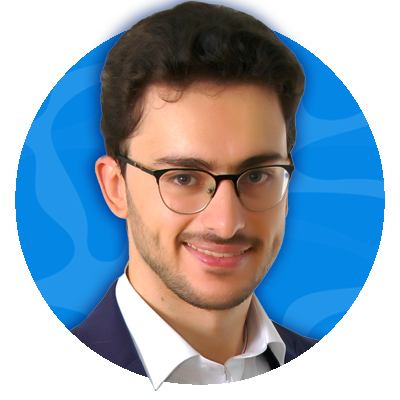
\includegraphics[width=0.9\textwidth]{images/example.png}}
        \caption{Single image}
        \label{img:single}   
        \end{figure}

        This is an example of a multiple image figure \ref{img:multiple}
        
        \begin{figure}[htbp]
        \begin{subfigure}[t]{0.5\linewidth}
        \centering
        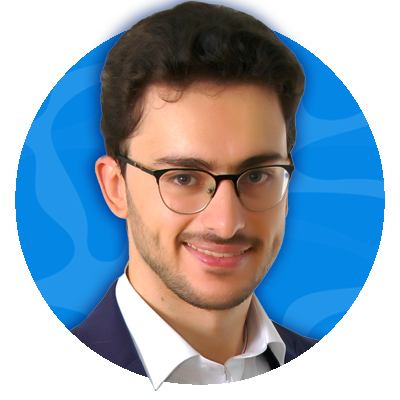
\includegraphics[width=0.7\textwidth]{images/example.png}
        \caption{Image 1}
        \label{subfig:img1}
        \end{subfigure}%
        \begin{subfigure}[t]{0.5\linewidth}
        \centering
        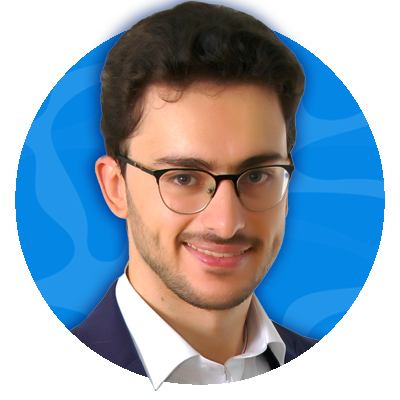
\includegraphics[width=0.7\textwidth]{images/example.png}
        \caption{Image 2}
        \label{subfig:img2}
        \end{subfigure}
        \caption{Multiple images}
        \label{img:multiple}
        \end{figure}
        
        
    \subsection{Tables}
        This is an example of a simple table \ref{tab:simple}

        \begin{table}[H]
        \centering
        \scalebox{1}{
        \begin{tabular}{|l|c|c|}
        \hline
        \textbf{x} & \textbf{y} & \textbf{z} \\
        \hline
        \textbf{a} & 5 & \cellcolor{green!10}7  \\
        \hline
        \textbf{b} & 63 & \cellcolor{green!10}8  \\
        \hline
        \end{tabular}
        }
        \caption{Simple table}
        \label{tab:simple}
        \end{table}

        This is an example of a complex table \ref{tab:complex}
        
        \begin{table}[htbp]
        \begin{center}
        
        \begin{tabular}{|c|l|c|c|c|}
        \cline{3-5}
        \multicolumn{2}{c|}{}&\multicolumn{3}{|c|}{\textbf{metric(\%)$\uparrow$}}\\
        \cline{2-5}
        \multicolumn{1}{c|}{}&\textbf{a} & train & valid & test  \\
        \hline
        
        \parbox[t]{2mm}{\multirow{2}{*}{\rotatebox[origin=c]{90}{\textbf{bc}}}}
        & b      &   5   &   5  &   5  \\
        & c      &   5   &   5  &   5  \\
        \hline
        \hline
        
        \parbox[t]{2mm}{\multirow{2}{*}{\rotatebox[origin=c]{90}{\textbf{de}}}} 
        & d      &   5  &   5   &   5  \\
        & e            &   5   &   5   &   5  \\
        \hline
        \hline   

        \rowcolor{gray!10}&\textbf{f} &   \textbf{10}   &   \textbf{10}   &   \textbf{10} \\
        \hline
        
        \end{tabular}
        \caption{Complex table}
        \label{tab:complex}
        \end{center}
        \end{table}


        
\section*{Conclusion}
    We presented ....

\chapter{Chapter 2}
\minitoc
\label{chap:2nd}

\section*{Introduction}
    This chapter outlines ...

\section*{Conclusion}
    In this chapter, we ....

\chapter{Chapter 3}
\minitoc
\label{chap:3rd}
\section*{Introduction}
    This chapter delves 
\section*{Conclusion}
    In this section, we...

\chapter{Chapter 4}
\minitoc
\label{chap:4th}
\section*{Introduction}
This chapter outlines ...


\section*{Conclusion}
    In this chapter, we ...

\chapter*{Conclusion and perspectives}
\label{conclusion}
\addcontentsline{toc}{chapter}{Conclusion and perspectives}
\markboth{Conclusion and perspectives}{}
\lettrine[findent=2pt]{\textbf{T}}{ }his is the general conclusion

\printbibliography[title=Bibliography, nottype=online]
\printbibliography[title=Webography, type=online]

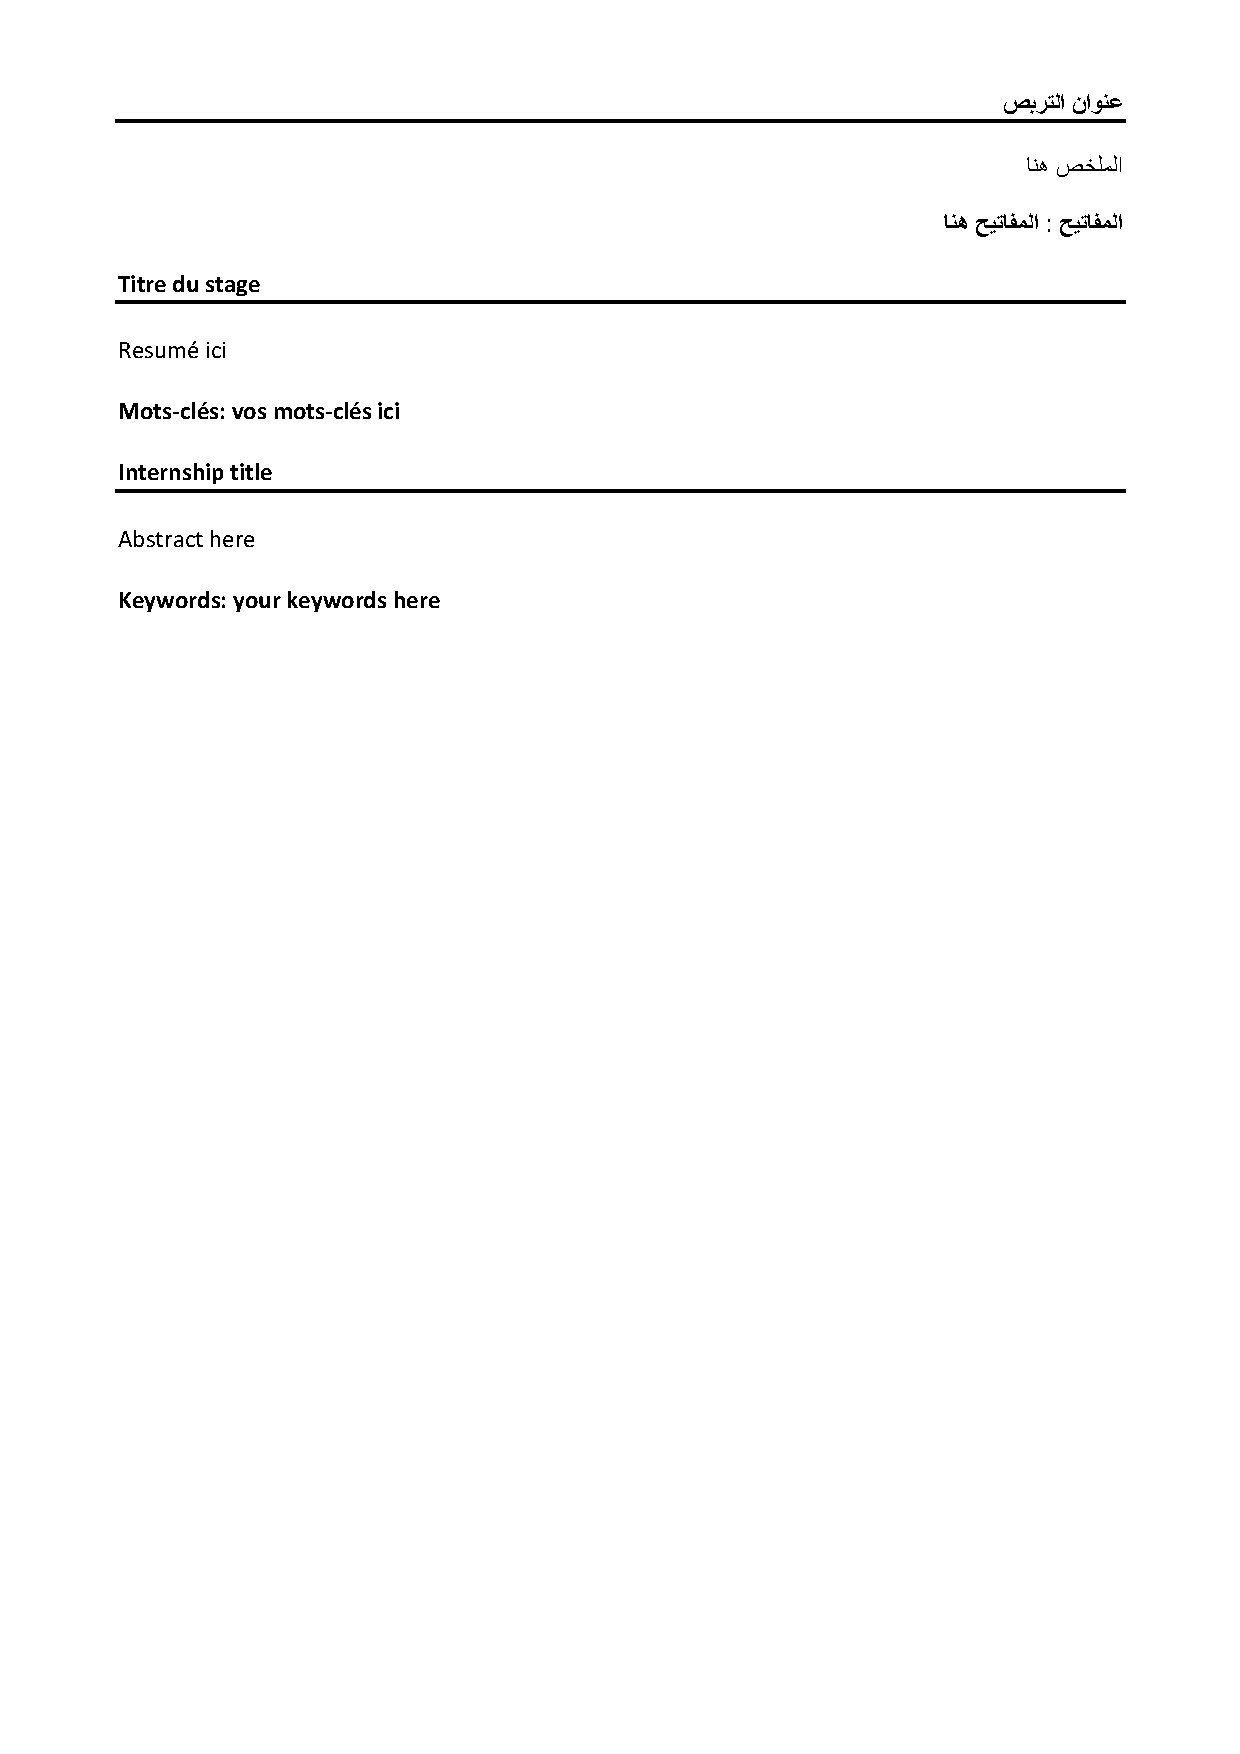
\includepdf[pages=-]{AbstractPage.pdf}


\end{document}